\documentclass[tikz,border=10pt]{standalone}
\usetikzlibrary{arrows.meta,positioning,fit}
\usepackage{xcolor}
\pagecolor{white}
\begin{document}
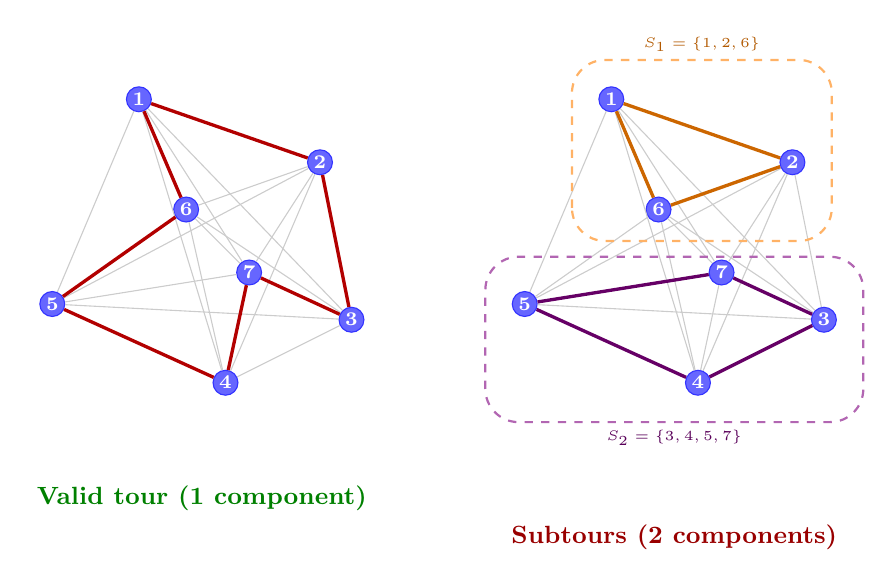
\begin{tikzpicture}[
  city/.style={circle, draw=blue!80, fill=blue!60, inner sep=0pt,
               minimum size=9pt, font=\scriptsize\bfseries, text=white},
  tour/.style={very thick, red!70!black},
  subtour/.style={very thick},
  nontour/.style={thin, gray!40},
  label/.style={font=\small\bfseries, below=8pt},
]
  % --- Valid tour (left) ---
  \begin{scope}
    \node[city] (a1) at (-0.3, 2.3)  {1};
    \node[city] (a2) at (2.0, 1.5)   {2};
    \node[city] (a3) at (2.4,-0.5)   {3};
    \node[city] (a4) at (0.8,-1.3)   {4};
    \node[city] (a5) at (-1.4,-0.3)  {5};
    \node[city] (a6) at (0.3, 0.9)   {6};
    \node[city] (a7) at (1.1, 0.1)   {7};

    % Faded complete graph
    \foreach \i in {1,...,7} {
      \foreach \j in {\i,...,7} {
        \ifnum\i<\j
          \draw[nontour] (a\i) -- (a\j);
        \fi
      }
    }

    % Tour: 1-6-5-4-7-3-2-1
    \draw[tour] (a1) -- (a6) -- (a5) -- (a4) -- (a7) -- (a3) -- (a2) -- (a1);

    \node[label, green!50!black] at (0.5, -2.2) {Valid tour (1 component)};
  \end{scope}

  % --- Subtours (right) ---
  \begin{scope}[xshift=6cm]
    \node[city] (b1) at (-0.3, 2.3)  {1};
    \node[city] (b2) at (2.0, 1.5)   {2};
    \node[city] (b3) at (2.4,-0.5)   {3};
    \node[city] (b4) at (0.8,-1.3)   {4};
    \node[city] (b5) at (-1.4,-0.3)  {5};
    \node[city] (b6) at (0.3, 0.9)   {6};
    \node[city] (b7) at (1.1, 0.1)   {7};

    % Faded complete graph
    \foreach \i in {1,...,7} {
      \foreach \j in {\i,...,7} {
        \ifnum\i<\j
          \draw[nontour] (b\i) -- (b\j);
        \fi
      }
    }

    % Subtour 1: {1, 2, 6}
    \draw[subtour, orange!80!black] (b1) -- (b6) -- (b2) -- (b1);

    % Subtour 2: {3, 4, 5, 7}
    \draw[subtour, violet!80!black] (b5) -- (b7) -- (b3) -- (b4) -- (b5);

    % Dashed ovals
    \draw[orange!60, thick, dashed, rounded corners=12pt]
      (-0.8, 0.5) rectangle (2.5, 2.8);
    \draw[violet!60, thick, dashed, rounded corners=12pt]
      (-1.9, -1.8) rectangle (2.9, 0.3);

    \node[font=\tiny, orange!70!black] at (0.85, 3.0) {$S_1 = \{1,2,6\}$};
    \node[font=\tiny, violet!70!black] at (0.5, -2.0) {$S_2 = \{3,4,5,7\}$};

    \node[label, red!60!black] at (0.5, -2.7) {Subtours (2 components)};
  \end{scope}
\end{tikzpicture}
\end{document}
